\chapter{静止作用とEuler--Lagrange方程式}

\lectureoverview{よく知られた\emph{最小作用の原理}という名は、本質的な点を覆い隠している。すなわち、物理的な軌道は作用を停留させるのであって、必ずしもそれを最小にする必要はない。この主張を通常の平衡から組み立て、点から関数全体へと拡張し、経路を離散化することによってオイラー--ラグランジュ方程式を導き、ニュートンの方程式を回復する。次に、回転座標と極座標によって、ラグランジュ形式が単なる表記の変更以上のものである理由を示す。}

\section{停留であって、必ずしも最小ではない}

伝統的な名において信頼できない部分は\emph{最小}という語である。古典的な軌道は常に作用を最小にするわけではない。代わりに、可能な軌道の空間において最大値または鞍点を与えることもある。正しい原理は、作用が\emph{停留}であること、すなわちその一次の変化が消えることである。

まず、より単純な平衡の問題から始めよう。静止し続ける粒子は加速度をもたないので、その正味の力は消えなければならない。一次元のポテンシャルから導かれる力に対して、
\begin{equation}
  F(x)=-\frac{dV}{dx},
  \label{eq:force-from-v}
\end{equation}
平衡条件は
\begin{equation}
  \frac{dV}{dx}=0.
  \label{eq:stationary-v-one}
\end{equation}

\begin{figure}[htbp]
  \centering
  \includegraphics[width=0.74\textwidth]{lecture_03_figure_02.png}
  \caption{一次元の平衡条件：ポテンシャルが停留する点で力が消える。}
  \lectureframe{00:02:51}
\end{figure}

次に、粒子を小さな量\(\delta x\)だけ変位させる。一次まででは、
\begin{equation}
  \delta V
  =V(x+\delta x)-V(x)
  =\frac{dV}{dx}\,\delta x+O(\delta x^2).
  \label{eq:first-variation-one}
\end{equation}
平衡では、\(\delta x\)のどちらの符号に対しても線形項はゼロである：
\begin{equation}
  \delta V=0
  \qquad\hbox{to first order.}
  \label{eq:delta-v-zero-one}
\end{equation}
これは、有限の移動の後で\(V\)が厳密に変わらないと言っているのではない。主要な変化が二次以上であると言っているのである。極小と極大はどちらもこの条件を満たす。

\begin{figure}[htbp]
  \centering
  \begin{tikzpicture}[scale=0.95,>=Latex]
    \draw[->] (-0.2,0) -- (3.35,0) node[right] {$x$};
    \draw[->] (0,-0.2) -- (0,2.25) node[above] {$V$};
    \draw[blue!65!black,thick,smooth]
      plot coordinates {(0.2,1.85) (0.75,0.85) (1.55,0.35)
                        (2.35,0.85) (3.0,1.85)};
    \fill[red!65!black] (1.55,0.35) circle (2pt);
    \node at (1.55,-0.34) {minimum};
    \begin{scope}[xshift=4.25cm]
      \draw[->] (-0.2,0) -- (3.35,0) node[right] {$x$};
      \draw[->] (0,-0.2) -- (0,2.25) node[above] {$V$};
      \draw[blue!65!black,thick,smooth]
        plot coordinates {(0.2,0.35) (0.75,1.25) (1.55,1.85)
                          (2.35,1.25) (3.0,0.35)};
      \fill[red!65!black] (1.55,1.85) circle (2pt);
      \node at (1.55,-0.34) {maximum};
    \end{scope}
  \end{tikzpicture}
  \caption{停留性が定めるのは一次導関数であり、その点が極小か極大かではない。}
  \label{fig:min-max-stationary}
\end{figure}

多くの座標\(q_i\)に対して、一次変分は
\begin{equation}
  \delta V
  =\sum_i\frac{\partial V}{\partial q_i}\,\delta q_i.
  \label{eq:first-variation-many}
\end{equation}
これがすべての独立な無限小変位\(\delta q_i\)に対して消えなければならないなら、すべての係数が消える：
\begin{equation}
  \frac{\partial V}{\partial q_i}=0
  \qquad\hbox{for every }i.
  \label{eq:stationary-v-many}
\end{equation}

二次元のポテンシャルは、ジェットコースターというよりも起伏のある地形として想像する方がよい。停留点は谷底、山頂、または鞍点でありうる。鞍点では、ある方向の運動は最初に登り、別の方向の運動は最初に下る。したがって、その点自体ですべての一次導関数が消えていても、復元挙動は一方向では安定、別の方向では不安定になりうる。

\begin{figure}[htbp]
  \centering
  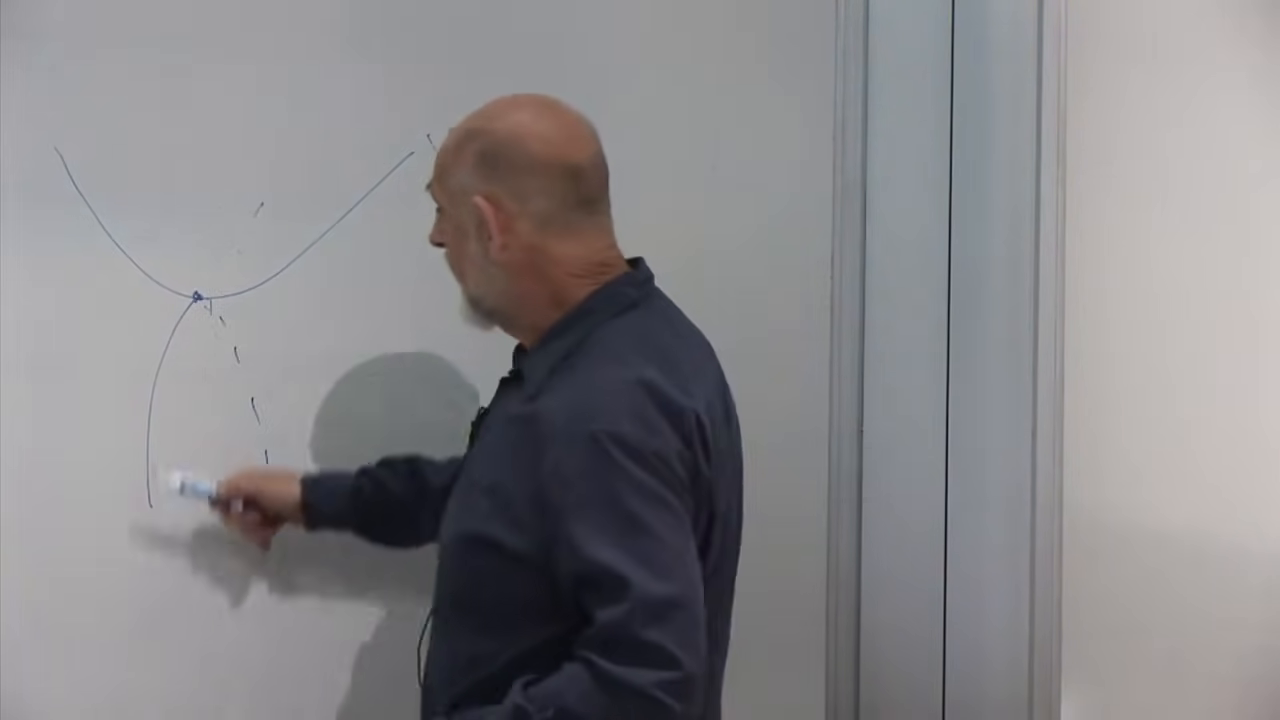
\includegraphics[width=0.76\textwidth]{lecture_03_figure_06.png}
  \caption{鞍点は、隣接する変位がある軸に沿って上昇し別の軸に沿って下降するにもかかわらず、すべての一次の方向で停留である。}
  \lectureframe{00:08:20}
\end{figure}

多くの座標をもつ空間では、鞍点は純粋な極大や極小よりも典型的である。これが、\emph{停留}が長く使える語である理由である。条件
\begin{equation}
  \delta V=0
  \label{eq:equilibrium-variation}
\end{equation}
は、二次の挙動を先取りすることなく平衡を要約している。

\section{点から関数へ}

力学は孤立した平衡点ではなく、運動全体を扱う。軌道は\(x(t)\)のような関数、または\((x(t),y(t),z(t))\)の集まりである。関数全体を変分してある量を停留させるという数学的問題は、\emph{変分法}である。これを運動に適用する前に、三つのより単純な例を考えよう。

\subsection{最短曲線と測地線}

平面上の二点を固定し、それらの間の曲線を\(y(x)\)で表す。短い線分にわたって、
\begin{equation}
  ds=\sqrt{dx^2+dy^2}
  =dx\sqrt{1+\left(\frac{dy}{dx}\right)^2},
  \label{eq:line-element}
\end{equation}
ここで最後の形は\(dx>0\)を仮定している。全長は汎関数
\begin{equation}
  S[y]=\int_{x_0}^{x_1}
  \sqrt{1+y'(x)^2}\,dx.
  \label{eq:arc-length-functional}
\end{equation}
である。角括弧は、\(S\)が関数全体を入力としてとることを強調している。直線は、両端点を固定したまま曲線を小さく変化させたときの
\begin{equation}
  \delta S=0
  \label{eq:stationary-length}
\end{equation}
によって選ばれる。

\begin{figure}[htbp]
  \centering
  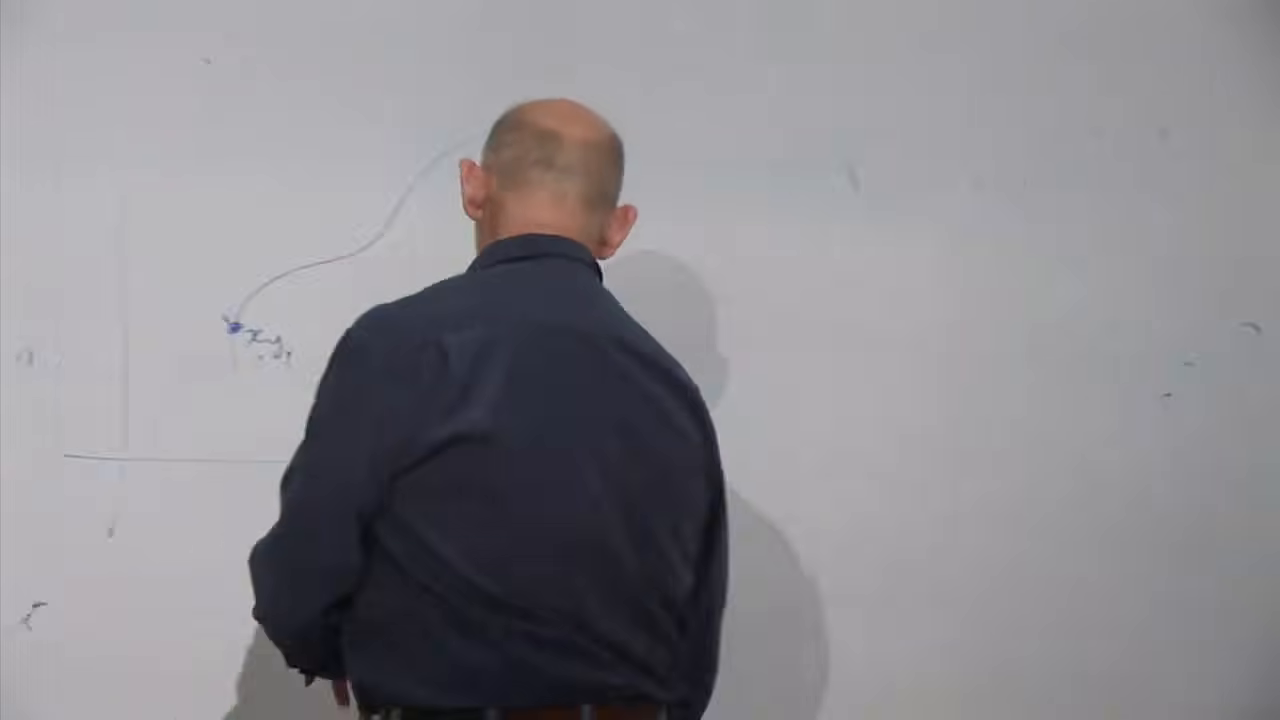
\includegraphics[width=0.78\textwidth]{lecture_03_figure_07.png}
  \caption{二つの固定端点の間の試行曲線。その長さは無限小の斜辺\(ds\)の和である。}
  \lectureframe{00:13:36}
\end{figure}

同じ問いは曲面上でも問うことができる。二本の杭の間に糸をぴんと張ると、拘束された最短経路の物理的な描像が得られる。そのような停留長の曲線は\emph{測地線}である。平らな平面上では直線であるが、球面や起伏のある曲面上では一般にはそうではない。

\subsection{Fermatの原理}

位置に依存する速さ\(c(x,y)\)をもつ媒質中の光線は、必ずしも空間的な最短経路に従う必要はない。小さな線分に要する時間は距離を局所的な速さで割ったものであるから、
\begin{equation}
  T[y]
  =\int_{x_0}^{x_1}
  \frac{\sqrt{1+y'(x)^2}}{c(x,y)}\,dx.
  \label{eq:fermat-functional}
\end{equation}
Fermatの原理は
\begin{equation}
  \delta T=0.
  \label{eq:fermat-stationary}
\end{equation}
を要求する。\(c\)が一定のとき、これは最短距離の問題に帰着する。しかし、屈折率が変化する媒質中では、最速の経路は距離と局所的な伝播速度を釣り合わせる。

\begin{figure}[htbp]
  \centering
  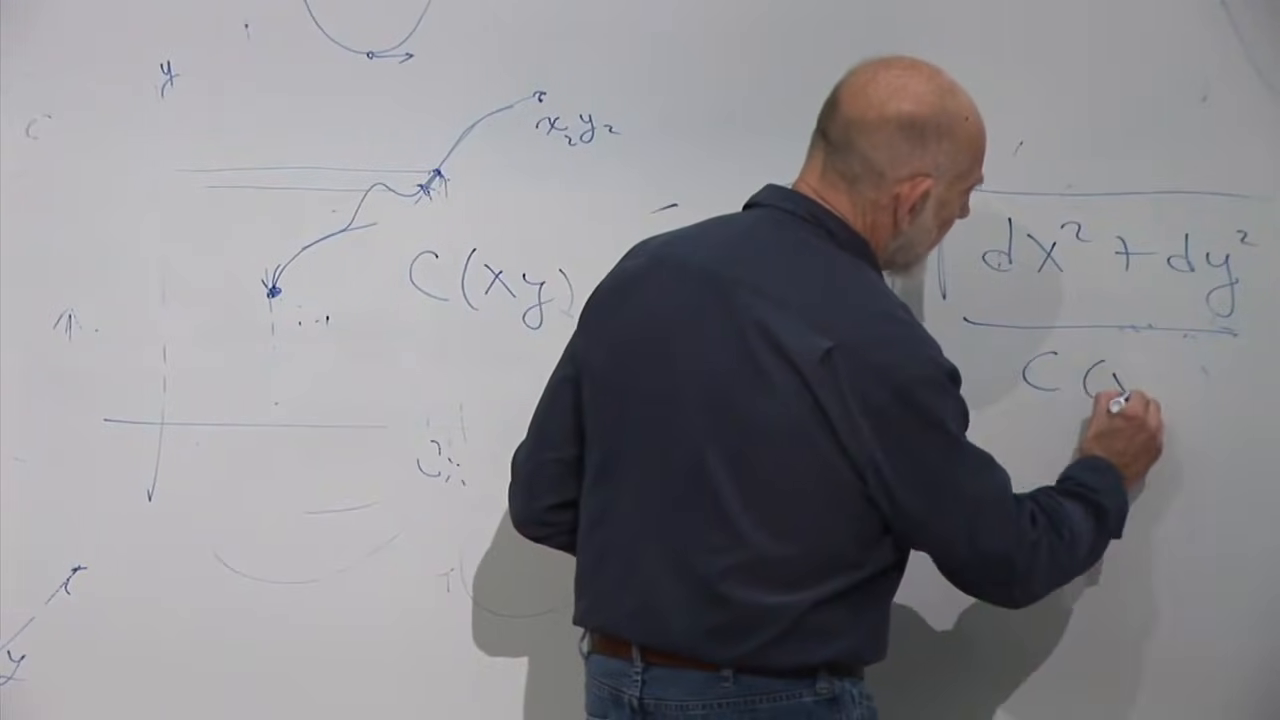
\includegraphics[width=0.80\textwidth]{lecture_03_figure_08.png}
  \caption{局所的な光速が位置に依存する媒質中を進む光線に対する最小時間の汎関数。}
  \lectureframe{00:22:50}
\end{figure}

時事ネタの冗談は、当時最近の主張、すなわちニュートリノがイタリアで異常に速く移動したという主張を引き合いに出す。物理学の議論は直ちに信頼できる例に戻る。すなわち、通常の光は屈折率に従って物質中で速度を変えるのである。

\subsection{吊り下げられた鎖}

二点で固定された鎖はカテナリーの形に落ち着く。各部分は重力による位置エネルギーに寄与するので、全位置エネルギーそれ自体が鎖に沿った積分である。ここでもまた端点は固定され、未知の形状は関数であり、積分が停留値を持たなければならない。

\begin{figure}[htbp]
  \centering
  \includegraphics[width=0.76\textwidth]{lecture_03_figure_03.png}
  \caption{固定された支持点の間に吊り下げられた鎖。その停留形状は全重力位置エネルギーによって選ばれる。}
  \lectureframe{00:30:41}
\end{figure}

これらの例は同じ構造を持つ。二つの固定された端点、その間の関数、そして第一変分が消える積分である。このような大域的な指示を微分方程式に還元することが、変分問題を解くという意味である。

\section{境界値問題としての力学}

軌道はしばしば時間を横軸にして描かれる。それは\(t\)が独立変数だからである。それにもかかわらず、物理学には時間を上向きに描くという強い慣習がある。余談として、若い頃から年を取るまでの写真を自分の書記体系に関連する方向に並べる実験が想起される。左から右へ読む人は左から右へ並べる傾向があり、右から左へ読む人は逆の方向に、縦書きに慣れた読者は縦に並べた。物理学者とは、時間は上向きに流れると主張する人々である、とその冗談は締めくくる。ここでは\(x(t)\)がグラフとして自然に読めるので、慣習的な水平な\(t\)軸を用いる。

初期値定式化では、\(t_0\)におけるデータは
\begin{equation}
  x(t_0)=x_0,
  \qquad
  \dot x(t_0)=v_0.
  \label{eq:initial-value-data}
\end{equation}
であり、ニュートンの方程式がその後の軌道を決定する。変分定式化は異なる問題を提起する。すなわち、二つの端点事象
\begin{equation}
  x(t_0)=x_0,
  \qquad
  x(t_1)=x_1,
  \label{eq:boundary-value-data}
\end{equation}
を指定し、それらの間の物理的な経路を決定するのである。初期速度はもはや与えられず、解の一部となる。

\begin{figure}[htbp]
  \centering
  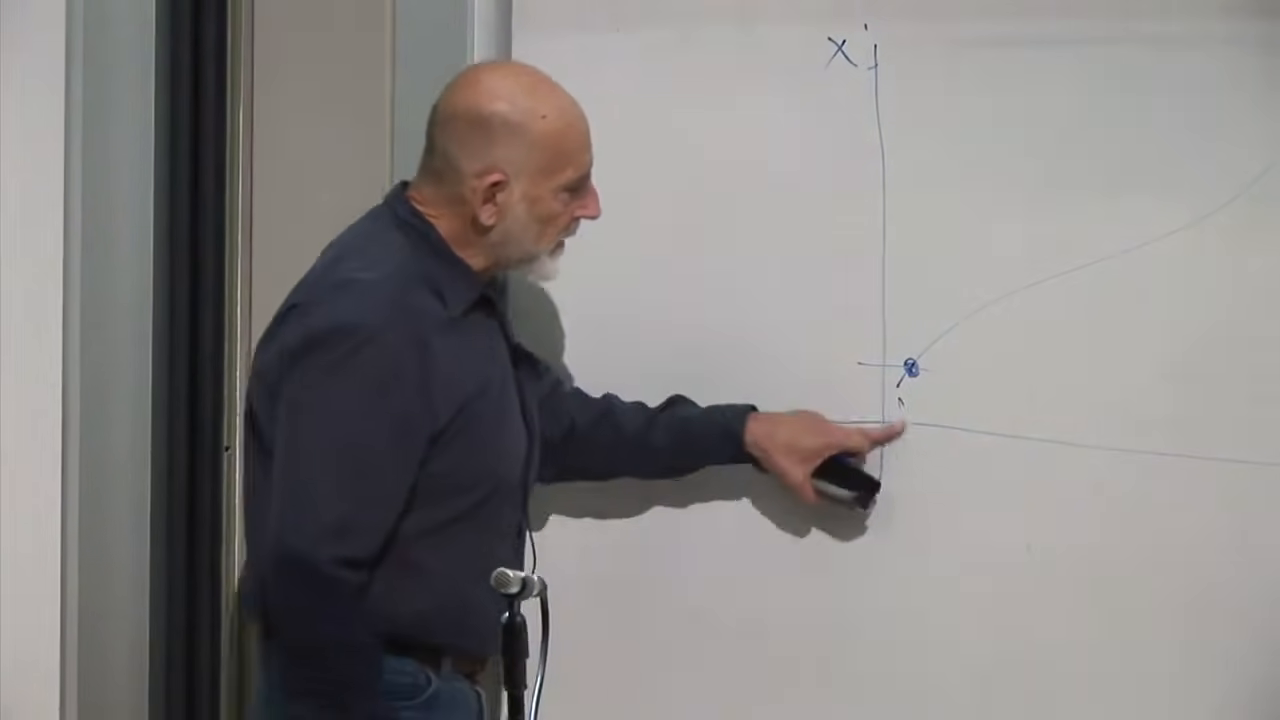
\includegraphics[width=0.76\textwidth]{lecture_03_figure_09.png}
  \caption{力学軌道\(x(t)\)。一端で位置と傾きを指定してもよいし、二つの端点時刻で位置を指定してもよい。}
  \lectureframe{00:27:41}
\end{figure}

停留値とすべき量は\emph{作用}
\begin{equation}
  A[x]=\int_{t_0}^{t_1}L(x,\dot x,t)\,dt.
  \label{eq:action-one}
\end{equation}
である。被積分関数\(L\)は\emph{ラグランジアン}である。それは位置、速度、そして陽に時間に依存しうる。作用原理は
\begin{equation}
  \delta A=0
  \label{eq:stationary-action}
\end{equation}
であり、
\begin{equation}
  \delta x(t_0)=\delta x(t_1)=0.
  \label{eq:fixed-endpoint-variations}
\end{equation}
を満たすすべての小さな経路の変分に対して成り立つ。端点条件は本質的である。すなわち、同じ二つの事象を結ぶ隣接する経路を比較するのである。

\section{オイラー--ラグランジュ方程式の離散的導出}

作用は無数の経路の値の汎関数である。その変分を具体的にするために、時間区間を長さ
\(\epsilon\)
の刻みに分割し、
\begin{equation}
  t_n=t_0+n\epsilon,
  \qquad
  x_n=x(t_n),
  \label{eq:discrete-times}
\end{equation}
第\(n\)区間における速度を
\begin{equation}
  v_n=\frac{x_{n+1}-x_n}{\epsilon}.
  \label{eq:discrete-velocity}
\end{equation}
で近似する。積分は通常の和
\begin{equation}
  A_\epsilon
  =\sum_{n=0}^{N-1}
  \epsilon L\left(x_n,\frac{x_{n+1}-x_n}{\epsilon}\right).
  \label{eq:discrete-action}
\end{equation}
となる。時間スライスのラベルには\(n\)を用いる。そうすれば\(i\)は後に空間座標と粒子のために取っておけるからである。

\begin{figure}[htbp]
  \centering
  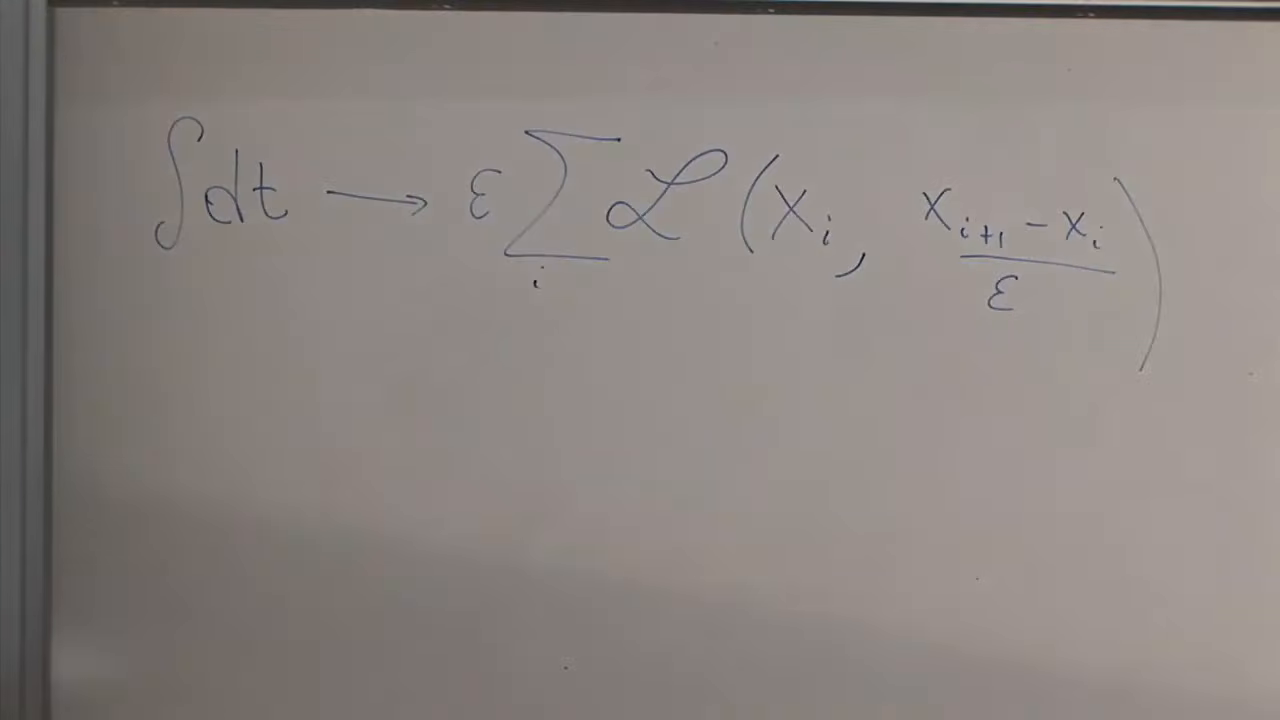
\includegraphics[width=0.82\textwidth]{lecture_03_figure_10.png}
  \caption{軌道を時間スライスの連鎖で置き換えたもの。一つの内部の高さを変えると、その隣接する二つの線分だけが変化する。}
  \lectureframe{00:38:30}
\end{figure}

一つの内部点\(x_n\)を変え、他のすべての\(x_k\)を固定する。和の中で\(x_n\)に依存する項は二つだけである。
\begin{align}
  A_\epsilon\big|_{x_n}
  &=
  \epsilon L\left(x_n,\frac{x_{n+1}-x_n}{\epsilon}\right)
  \notag\\
  &\quad+
  \epsilon L\left(x_{n-1},
                  \frac{x_n-x_{n-1}}{\epsilon}\right).
  \label{eq:two-neighbor-terms}
\end{align}
微分すると
\begin{align}
  0=\frac{\partial A_\epsilon}{\partial x_n}
  &=
  \epsilon\frac{\partial L_n}{\partial x_n}
  -\frac{\partial L_n}{\partial v_n}
  +\frac{\partial L_{n-1}}{\partial v_{n-1}}.
  \label{eq:discrete-el-variation}
\end{align}
が得られる。逆符号は単純な幾何学的起源を持つ。\(x_n\)を上げると、その後ろの区間の傾きが増し、その先の区間の傾きが減るのである。

\begin{figure}[htbp]
  \centering
  \includegraphics[width=0.74\textwidth]{lecture_03_figure_04.png}
  \caption{離散変分における直接の位置微分と、隣接する二つの速度微分の寄与。}
  \lectureframe{00:45:26}
\end{figure}

式~\eqref{eq:discrete-el-variation}を整理すると
\begin{equation}
  \frac{1}{\epsilon}
  \left(
    \frac{\partial L_n}{\partial v_n}
    -\frac{\partial L_{n-1}}{\partial v_{n-1}}
  \right)
  =
  \frac{\partial L_n}{\partial x_n}.
  \label{eq:discrete-el}
\end{equation}
左辺は隣接する差分商である。
\(\epsilon\to0\)
とすると、折れ線は滑らかな経路になり、商は時間微分になる。
\begin{equation}
  \boxed{
  \frac{d}{dt}\left(\frac{\partial L}{\partial\dot x}\right)
  =
  \frac{\partial L}{\partial x}}
  .
  \label{eq:euler-lagrange-one}
\end{equation}
これがオイラー--ラグランジュ方程式である。

\begin{figure}[htbp]
  \centering
  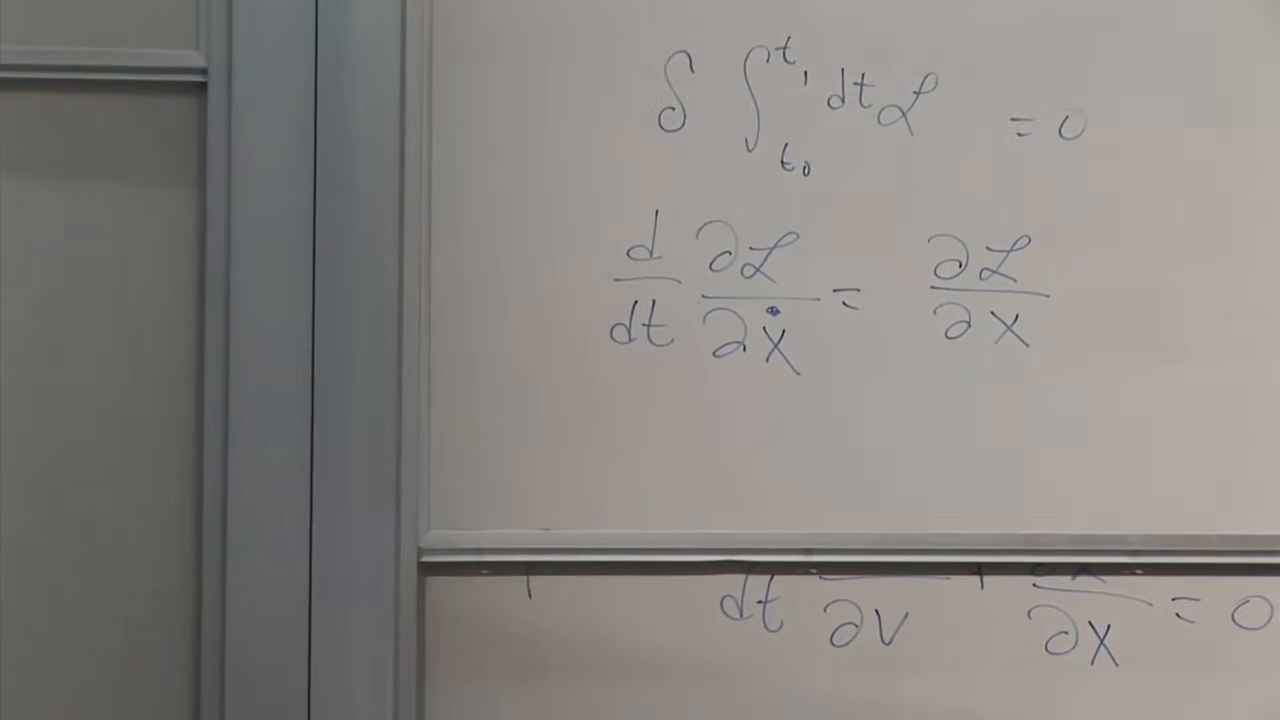
\includegraphics[width=0.78\textwidth]{lecture_03_figure_11.png}
  \caption{各内部時間スライスにおける停留性から得られる、完成したオイラー--ラグランジュ方程式。}
  \lectureframe{00:49:25}
\end{figure}

\(L\)が指定されれば、式~\eqref{eq:euler-lagrange-one}は機械として働く。すなわち、与えられた関数を微分すれば、その機械は経路に対する微分方程式を返すのである。

\begin{classroomqa}
  \audiencequestion{Euler--Lagrangeの結果は、
  \(x\)と\(\dot x\)の任意の関数に対して成り立つか。\lecturetimestamp{00:49:37--00:50:24}}
  \lecturerresponse{はい、導関数に必要な正則性を条件として成り立つ。
  弧長の例は、その独立変数\(x\)を\(t\)が果たす役割と
  みなし、その未知関数\(y(x)\)を\(x(t)\)が果たす役割と
  みなして名前を付け替えると、まったく同じ形になる。
  そのEuler--Lagrange方程式は直線解をもつ。}
\end{classroomqa}

\section{LagrangianからのNewtonの方程式}

ポテンシャル\(V(x)\)中の直線上の粒子に対して、
\begin{equation}
  L(x,\dot x)=T-V
  =\frac12m\dot x^2-V(x).
  \label{eq:lagrangian-tv-one}
\end{equation}
をとる。全エネルギーは\(T+V\)であるから、負号は奇妙に見えるかもしれない。
しかしLagrangianはエネルギーではない。その試金石は、Euler--Lagrangeの仕組みが
正しい運動を返すかどうかである。負号についての模擬投票は断る。
答えは選挙で決めるのではなく、検証されなければならない。

まず、
\begin{equation}
  \frac{\partial L}{\partial\dot x}=m\dot x.
  \label{eq:conjugate-momentum-one}
\end{equation}
これは運動量である。より一般に、任意の座標\(q\)に共役な運動量は
\begin{equation}
  p_q=\frac{\partial L}{\partial\dot q}.
  \label{eq:conjugate-momentum-general}
\end{equation}
で定義される。式~\eqref{eq:conjugate-momentum-one}の時間微分をとると
\(m\ddot x\)が得られ、一方
\begin{equation}
  \frac{\partial L}{\partial x}
  =-\frac{dV}{dx}.
  \label{eq:lagrangian-position-derivative}
\end{equation}
である。したがってEuler--Lagrange方程式は
\begin{equation}
  m\ddot x=-\frac{dV}{dx}=F(x),
  \label{eq:newton-from-action}
\end{equation}
となり、これはNewtonの第2法則である。

\begin{figure}[htbp]
  \centering
  \includegraphics[width=0.80\textwidth]{lecture_03_figure_05.png}
  \caption{運動エネルギー、ポテンシャルエネルギー、\(L=T-V\)、および復元された
  Newtonの方程式の成分形を1つの板書にまとめたもの。}
  \lectureframe{00:57:52}
\end{figure}

多くの座標\(q_i\)に対して、
\begin{equation}
  L(\mathbf q,\dot{\mathbf q})
  =\sum_i\frac12m_i\dot q_i^{\,2}-V(q_1,q_2,\ldots),
  \label{eq:lagrangian-tv-many}
\end{equation}
であり、各座標について1つの方程式がある。
\begin{equation}
  \frac{d}{dt}\left(\frac{\partial L}{\partial\dot q_i}\right)
  =\frac{\partial L}{\partial q_i}
  \quad\Longrightarrow\quad
  m_i\ddot q_i=-\frac{\partial V}{\partial q_i}=F_i.
  \label{eq:euler-lagrange-many}
\end{equation}
軌道は依然として1つの曲線であり、今度は高次元の
配置空間を通る。

\begin{classroomqa}
  \audiencequestion{我々は単にNewtonの法則から逆算して、
  答えを再現する汎関数を人為的に作っただけではないのか。\lecturetimestamp{00:58:07--01:00:04}}
  \lecturerresponse{それは生産的な観点ではない。Lagrangianは
  物理系の簡潔な指定である。すなわち、すべての
  座標と速度の1つの関数が、その運動方程式のすべてをまとめ上げる。新しい
  理論では、物理学者は通常、作用を提案して方程式を導出し、
  すべての方程式を別々に推測したりはしない。}
\end{classroomqa}

このパッケージ化が一つの利点である。座標の自由度もまたもう一つの利点である。直線が最短であるという主張は、平面がデカルト座標、極座標、曲線座標のいずれで記述されるかに依存しない。同様に、作用の停留性は座標に依存しない。ただし\(L\)の式とそれから得られる成分方程式は変化する。

\section{回転木馬から見た自由粒子}

\((x,y)\)を慣性系のCartesian座標とし、\((X,Y)\)が角速度\(\omega\)で
一様に回転するとする。ここで用いる向きでは、
\begin{align}
  x&=X\cos\omega t+Y\sin\omega t,
  \notag\\
  y&=-X\sin\omega t+Y\cos\omega t.
  \label{eq:rotating-coordinate-map}
\end{align}
両系の間の角度は\(\omega t\)である。

\begin{figure}[htbp]
  \centering
  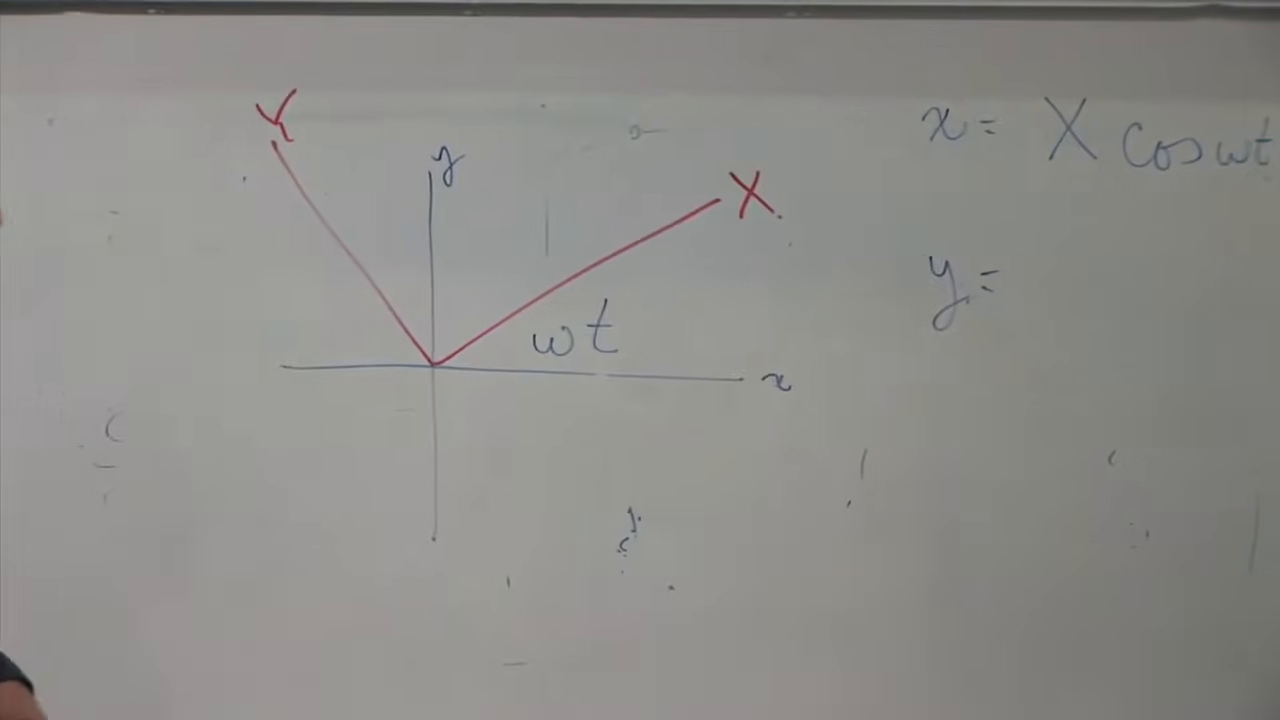
\includegraphics[width=0.76\textwidth]{lecture_03_figure_12.png}
  \caption{慣性系と一様回転するCartesian軸。同じ点が
  時間に依存する回転座標を受け取る。}
  \lectureframe{01:06:05}
\end{figure}

自由粒子は慣性系でLagrangian
\begin{equation}
  L_{\mathrm{in}}
  =\frac{m}{2}\left(\dot x^2+\dot y^2\right).
  \label{eq:free-inertial-lagrangian}
\end{equation}
をもつ。式~\eqref{eq:rotating-coordinate-map}を微分し、
\(\sin^2\omega t+\cos^2\omega t=1\)を用いる。三角関数の項が組み合わさって
\begin{align}
  \dot x^2+\dot y^2
  &=
  \dot X^2+\dot Y^2\\
  &\quad+\omega^2(X^2+Y^2)\\
  &\quad+2\omega(Y\dot X-X\dot Y).
  \label{eq:rotating-speed}
\end{align}
を与える。したがって
\begin{align}
  L_{\mathrm{rot}}
  &=
  \frac{m}{2}(\dot X^2+\dot Y^2)\\
  &\quad+\frac{m\omega^2}{2}(X^2+Y^2)\\
  &\quad+m\omega(Y\dot X-X\dot Y).
  \label{eq:rotating-lagrangian}
\end{align}

\begin{figure}[htbp]
  \centering
  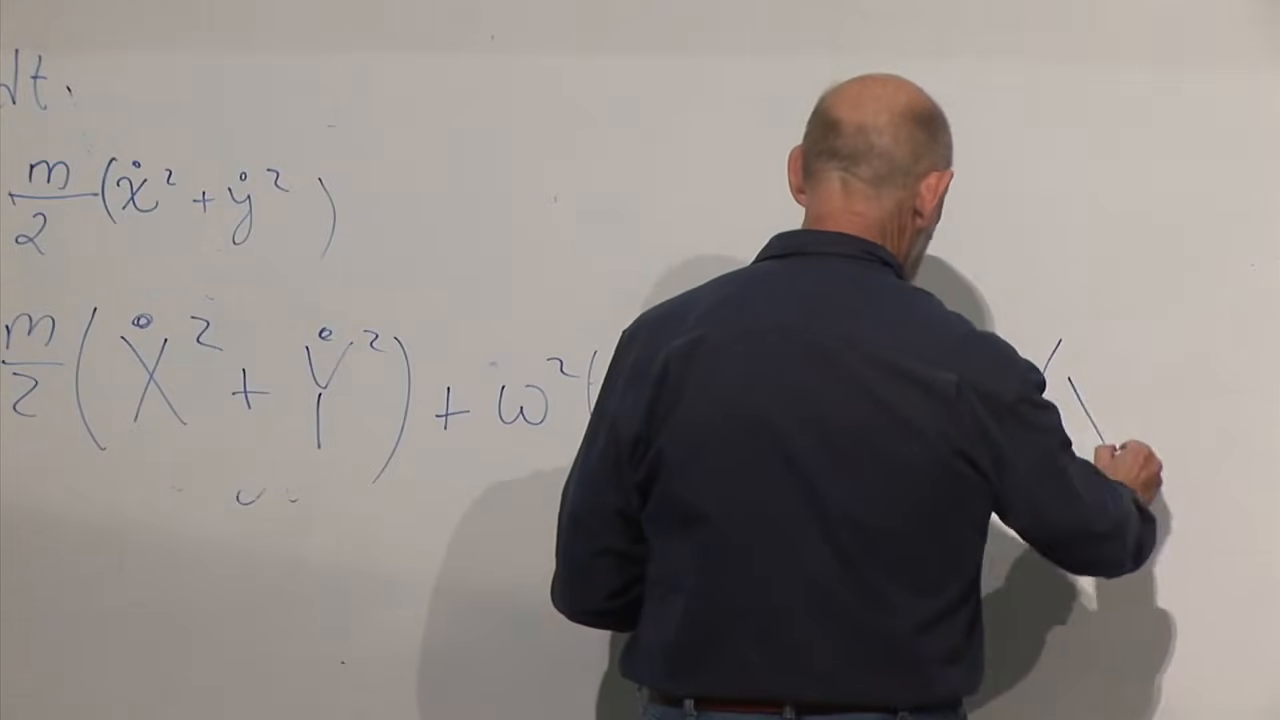
\includegraphics[width=0.84\textwidth]{lecture_03_figure_13.png}
  \caption{変換後の自由粒子ラグランジアン：通常の運動エネルギー、二次の遠心力項、速度に線形な項。}
  \lectureframe{01:12:16}
\end{figure}

二次の座標項は\(-V_{\mathrm{fict}}\)の形をとる。ここで
\begin{equation}
  V_{\mathrm{fict}}
  =-\frac{m\omega^2}{2}(X^2+Y^2).
  \label{eq:centrifugal-potential}
\end{equation}
これは外向きに減少するので、遠心力
\(m\omega^2(X,Y)\)を生じる。

式~\eqref{eq:rotating-lagrangian}の最後の項は座標と速度の両方に線形である。
Euler--Lagrange方程式を適用すると
\begin{align}
  m\ddot X&=m\omega^2X-2m\omega\dot Y,
  \notag\\
  m\ddot Y&=m\omega^2Y+2m\omega\dot X.
  \label{eq:rotating-equations}
\end{align}
が得られる。\(\omega^2\)に比例する項は遠心力であり、
速度に比例する項はCoriolisである。回転面内でのベクトル形では、
\begin{equation}
  \mathbf F_{\mathrm{C}}
  =-2m\,\boldsymbol\omega\times\mathbf v_{\mathrm{rot}},
  \label{eq:coriolis-vector}
\end{equation}
であり、逆向きの向きの規約を選ぶ場合は符号が調整される。

\begin{figure}[htbp]
  \centering
  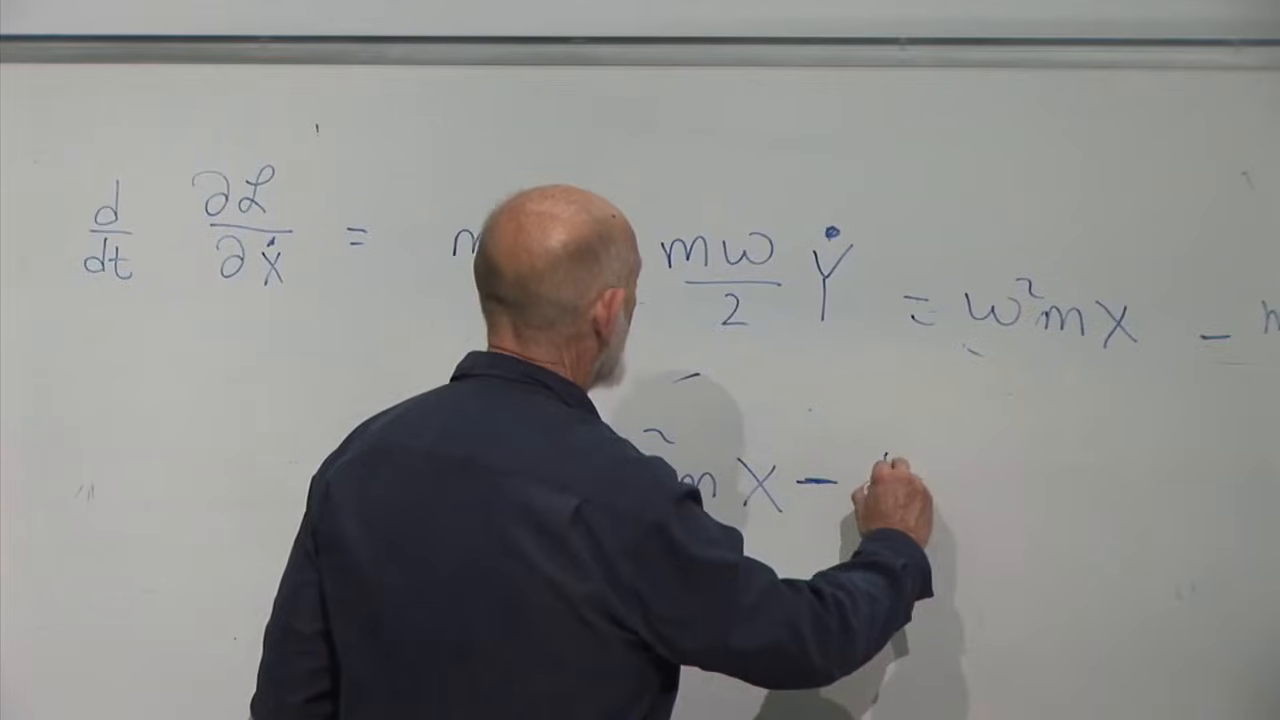
\includegraphics[width=0.84\textwidth]{lecture_03_figure_14.png}
  \caption{回転系の方程式。ここでは座標に比例する項が
  遠心加速度を与え、速度とのクロス項が
  Coriolis加速度を与える。}
  \lectureframe{01:20:20}
\end{figure}

要点は代数が消えることではない。一つのスカラー関数の一回の座標変換が、連立方程式と二つの見かけの力の両方を生み出すことである。

\begin{classroomqa}
  \audiencequestion{この方法は任意に曲がった
  座標に対しても機能するか。\lecturetimestamp{01:22:01--01:22:17}}
  \lecturerresponse{はい。新しい座標は曲線座標であってもよく、回転座標がそうであるように
  時間に陽に依存してもよい。作用を新しい変数で書き直し、同じEuler--Lagrangeの規則を適用すればよい。}
\end{classroomqa}

\section{極座標と巡回する角度}

通常の極座標では，
\begin{equation}
  x=r\cos\theta,
  \qquad
  y=r\sin\theta.
  \label{eq:polar-map}
\end{equation}
\(r\) と \(\theta\) はともに時間とともに変化しうる。微分して平方を加えると，
\begin{equation}
  \dot x^2+\dot y^2
  =\dot r^2+r^2\dot\theta^2.
  \label{eq:polar-speed}
\end{equation}
中心ポテンシャル \(V(r)\) に対して，
\begin{equation}
  L
  =\frac{m}{2}\left(\dot r^2+r^2\dot\theta^2\right)-V(r).
  \label{eq:polar-lagrangian}
\end{equation}

\begin{figure}[htbp]
  \centering
  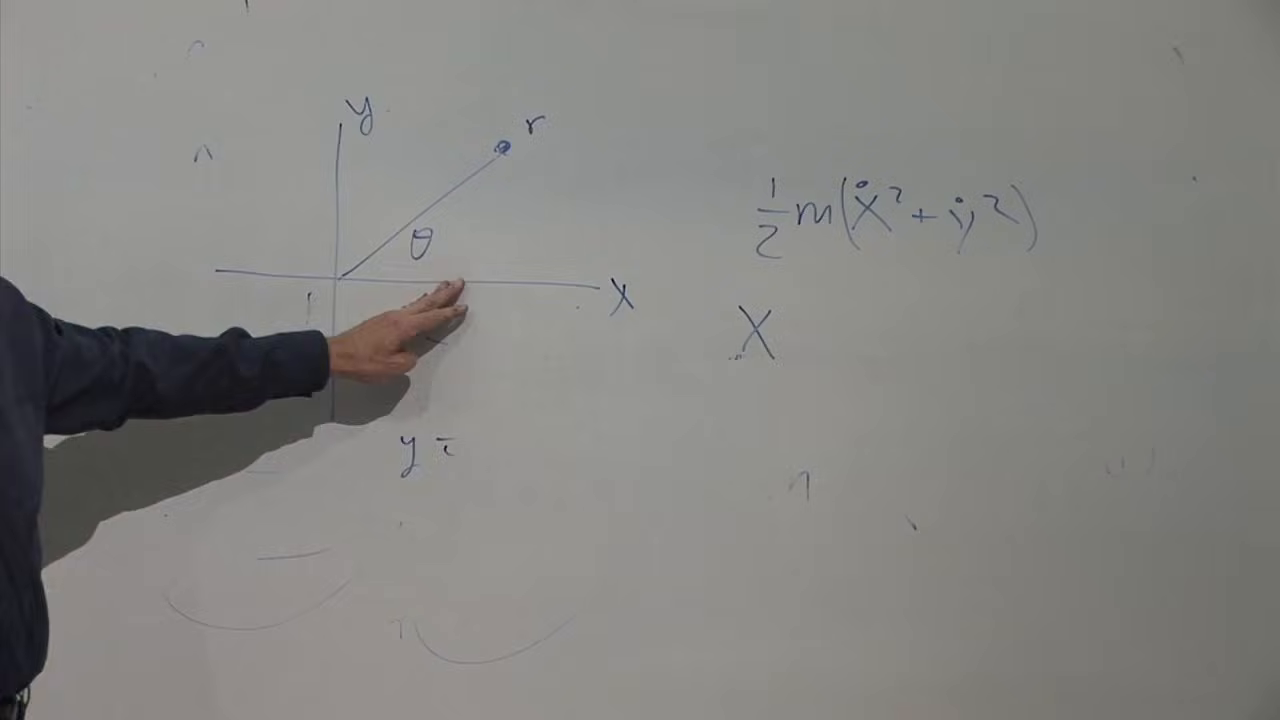
\includegraphics[width=0.80\textwidth]{lecture_03_figure_15.png}
  \caption{極座標の幾何と，運動エネルギーを動径運動と角運動に分解すること。}
  \lectureframe{01:23:30}
\end{figure}

動径方程式は
\begin{equation}
  m\ddot r
  =mr\dot\theta^2-\frac{dV}{dr}.
  \label{eq:radial-equation}
\end{equation}
第一項は，粒子自身の角運動に伴う外向きの遠心力寄与である。

角度については，
\begin{equation}
  \frac{d}{dt}\left(\frac{\partial L}{\partial\dot\theta}\right)
  =\frac{\partial L}{\partial\theta}=0,
  \label{eq:theta-el}
\end{equation}
なぜなら中心ポテンシャルは \(\theta\) に陽に依存しないからである。したがって
\begin{equation}
  \frac{d}{dt}\left(mr^2\dot\theta\right)=0,
  \qquad
  mr^2\dot\theta=\ell,
  \label{eq:angular-momentum}
\end{equation}
ここで \(\ell\) は保存する角運動量である。

\begin{figure}[htbp]
  \centering
  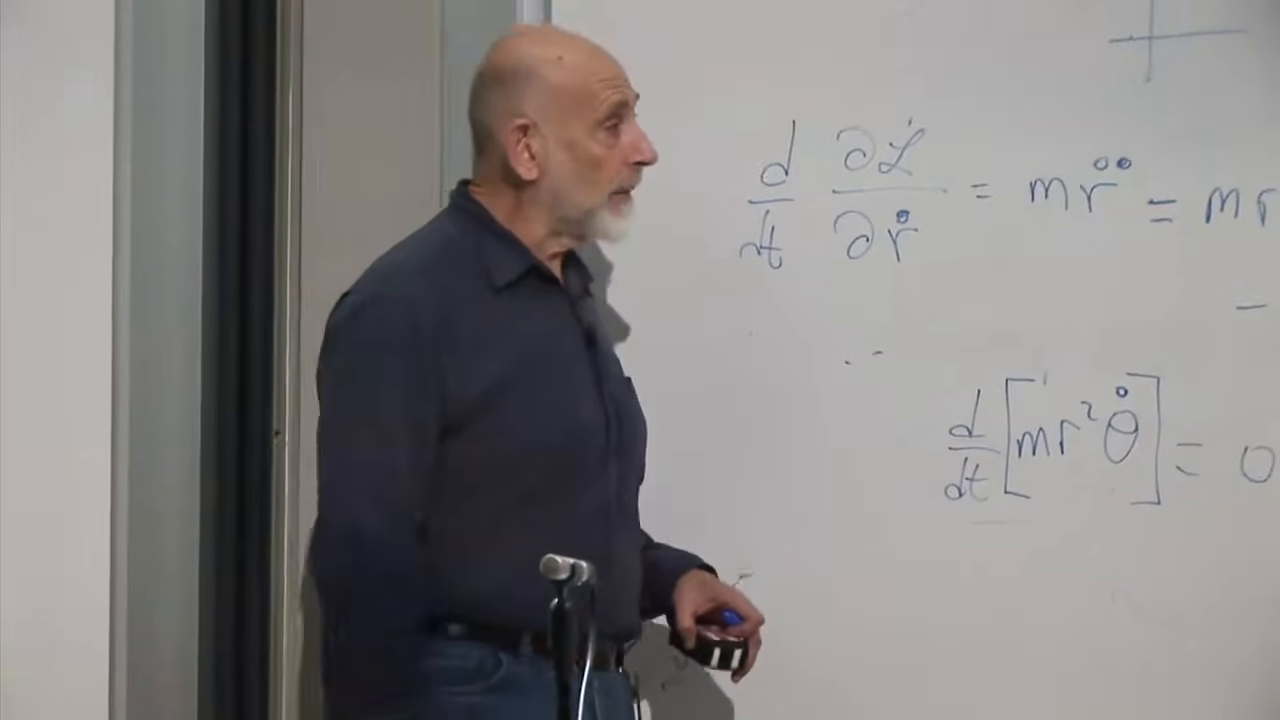
\includegraphics[width=0.82\textwidth]{lecture_03_figure_16.png}
  \caption{角に関する Euler--Lagrange 方程式の右辺はゼロであり，\(mr^2\dot\theta\) の保存を露わにする。}
  \lectureframe{01:29:25}
\end{figure}

角方程式から
\begin{equation}
  \dot\theta=\frac{\ell}{mr^2}.
  \label{eq:theta-dot-angular-momentum}
\end{equation}
が得られる。式~\eqref{eq:radial-equation}に代入すると，\(r\) に関する単一の方程式が残る：
\begin{equation}
  m\ddot r
  =\frac{\ell^2}{mr^3}-\frac{dV}{dr}.
  \label{eq:effective-radial-equation}
\end{equation}

\(L\) に現れない座標は，たとえ角度でなくても，伝統的に \emph{循環} と呼ばれる。\(q\) が循環的ならば，
\begin{equation}
  \frac{\partial L}{\partial q}=0
  \quad\Longrightarrow\quad
  \frac{d}{dt}\left(\frac{\partial L}{\partial\dot q}\right)=0.
  \label{eq:cyclic-conservation}
\end{equation}
その共役運動量は保存する。これは，対称性と保存則の一般的な結びつきの最初の手がかりである。

\section{意味，エネルギー，適用範囲に関する問い}

以下に続く問いは，この形式のより深い内容がどこにあるかを明らかにする。

\begin{classroomqa}
  \audiencequestion{正しい古典的方程式を与えると分かったというだけでなく、ラグランジアンに到達すべき独立の理由はあるのでしょうか。\lecturetimestamp{01:33:25--01:35:07}}
  \lecturerresponse{歴史的には、一世紀以上にわたる古典力学によって、粒子、波、電磁場のいずれもがこの形式で表されうることが示されてきました。古典的レベルでは、この積み重ねられた成功は、法則がどのように組織されるかについての経験的事実です。より深い説明は量子力学からもたらされるものであり、ここでは保留します。}
\end{classroomqa}

\begin{classroomqa}
  \audiencequestion{回転系の Lagrangian において，速度に線形な項に通常の運動エネルギーやポテンシャルエネルギーを割り当てることはできるか。\lecturetimestamp{01:35:08--01:36:23}}
  \lecturerresponse{いいえ。時間並進に対応する保存量は，Hamiltonian の構成によって得られるのであり，\(L\) のすべての項を運動エネルギーやポテンシャルエネルギーとして読むことによってではない。式~\eqref{eq:rotating-lagrangian}については，速度に線形な項は \(\sum_a\dot q_a\,\partial L/\partial\dot q_a-L\) から相殺される。Hamiltonian による扱いがこれを体系的に整理するであろう。}
\end{classroomqa}

実際，\(L_{\mathrm{rot}}\) は陽に時間に依存しないので，
\begin{equation}
  \begin{aligned}
    H_{\mathrm{rot}}
    &=\dot X\frac{\partial L}{\partial\dot X}
     +\dot Y\frac{\partial L}{\partial\dot Y}-L\\
    &=\frac{m}{2}(\dot X^2+\dot Y^2)
     -\frac{m\omega^2}{2}(X^2+Y^2)
  \end{aligned}
  \label{eq:rotating-hamiltonian-preview}
\end{equation}
は保存する。これは回転系の Jacobi 積分であり，慣性系の観測者が割り当てる同じ数値のエネルギーではない。時間に依存する座標変換は，エネルギーの数値的な形を必ずしも保たない。

\begin{classroomqa}
  \audiencequestion{曲がった軌道が重力によって引き起こされる場合はどうか。\lecturetimestamp{01:36:30--01:37:10}}
  \lecturerresponse{Newton 重力に対しては，中心力 Lagrangian において \(V(r)=-GMm/r\) をそのまま用いればよい。曲がった時空は一般相対論に属し，ここでは仮定しない。}
\end{classroomqa}

\begin{classroomqa}
  \audiencequestion{遠心力ポテンシャルとそのエネルギーは単に仮想的なものにすぎないのか。\lecturetimestamp{01:37:13--01:40:14}}
  \lecturerresponse{回転台上の観測者は有効力を測定し，回転系の保存量を矛盾なく用いることができる。\emph{仮想}とは，これらの項が非慣性系の記述から生じるという意味であり，観測される効果が想像上のものであるという意味ではない。エネルギーそれ自体は，一般の時間に依存する座標変換の下で不変ではない。}
\end{classroomqa}

\begin{classroomqa}
  \audiencequestion{速度に依存する Coriolis 力はどの方向を向くのか。\lecturetimestamp{01:40:22--01:42:36}}
  \lecturerresponse{それは回転系の速度に垂直であり，その大きさは速さと系の角速度に比例する。平面内では，式~\eqref{eq:rotating-equations}のように，成分が \(\dot X\) と \(\dot Y\) を逆符号で入れ替える。}
\end{classroomqa}

\begin{figure}[htbp]
  \centering
  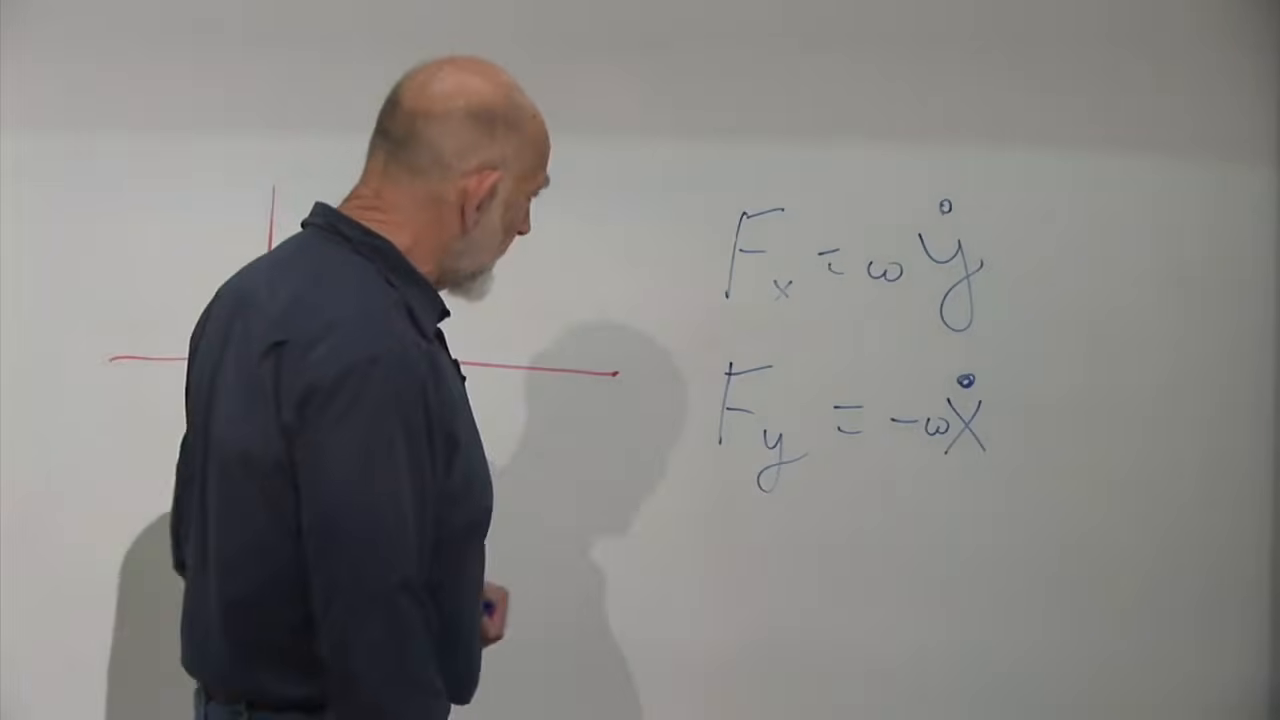
\includegraphics[width=0.76\textwidth]{lecture_03_figure_17.png}
  \caption{速度に直交する成分のパターン：Coriolis 力は回転系の速度に垂直である。}
  \lectureframe{01:41:40}
\end{figure}

\begin{classroomqa}
  \audiencequestion{出発点の Lagrangian は慣性系で書かれなければならないのか。\lecturetimestamp{01:42:37--01:44:00}}
  \lecturerresponse{通常の自由粒子に対しては，Newton の慣性系の法則が単純な出発形 \(m(\dot x^2+\dot y^2)/2\) を与える。ひとたびその物理法則が知られれば，作用は任意の他の座標へ変換できる。回転系において同じ単純な運動エネルギーの式を独立に仮定してはならない。}
\end{classroomqa}

同じ種類の速度に線形な項は，磁場中の荷電粒子に対しても現れる：
\begin{equation}
  L_{\mathrm{em}}
  =\frac12m\mathbf v^2
   +q\mathbf A(\mathbf r,t)\cdot\mathbf v
   -q\phi(\mathbf r,t).
  \label{eq:electromagnetic-lagrangian}
\end{equation}
平面に垂直な一様磁場に対して，対称ゲージ \(\mathbf A=\tfrac12\mathbf B\times\mathbf r\) は \(X\dot Y-Y\dot X\) に比例する項を生じ，これは Coriolis 項と同じ代数的構造である。

\begin{figure}[htbp]
  \centering
  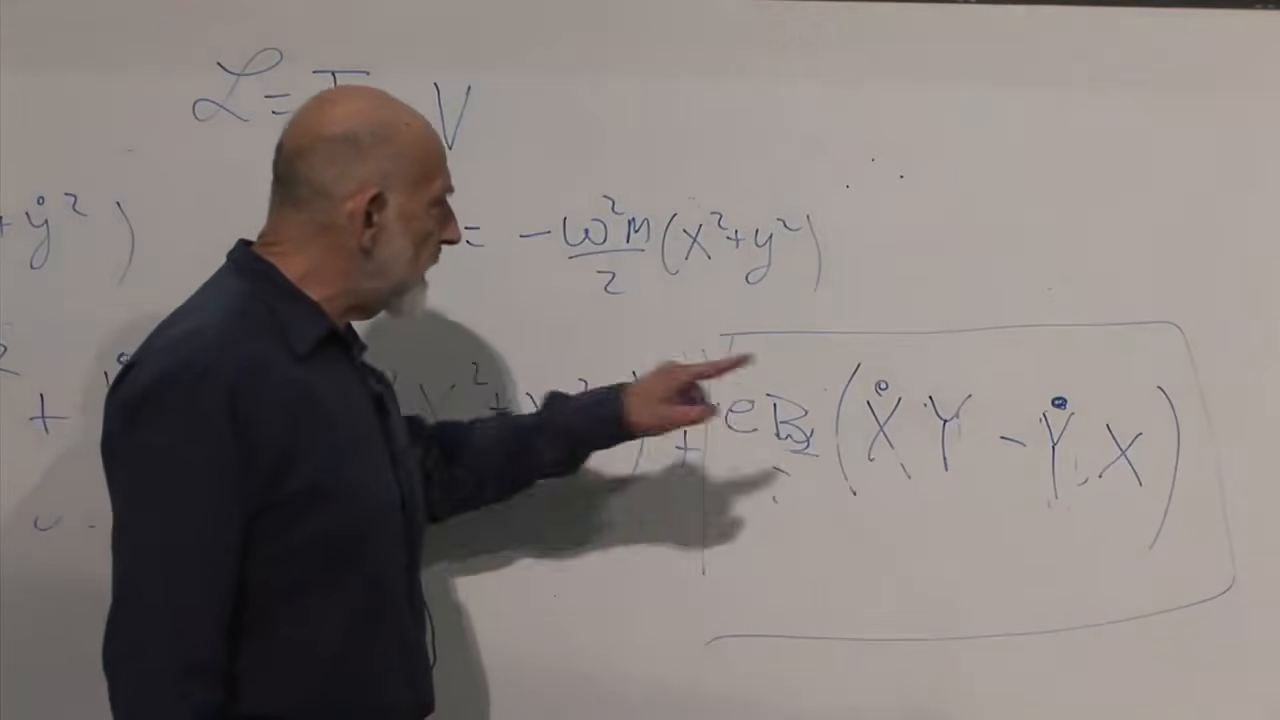
\includegraphics[width=0.82\textwidth]{lecture_03_figure_18.png}
  \caption{一様磁場中の荷電粒子との比較を動機づける、速度に線形な回転系の項。}
  \lectureframe{01:44:40}
\end{figure}

\begin{classroomqa}
  \audiencequestion{ラグランジアンとしてどのような関数が使えるかについて、滑らかさ以外に制約はあるのか。\lecturetimestamp{01:44:46--01:45:06}}
  \lecturerresponse{あるが、その関連する制約にはまだ展開されていないより多くの構造が必要であり、後回しにする。この段階での中心的な教訓は、提案されたラグランジアンがどのように方程式と保存則を生み出すかである。}
\end{classroomqa}

回転系の方程式は円運動も許容する。すなわち、慣性系に固定された点は、回転木馬から見ると回転原点の周りを円を描く。すると磁気との類推によって、荷電粒子がなぜ円形のサイクロトロン運動を行いうるかが説明される。

\begin{classroomqa}
  \audiencequestion{荷電粒子はその円上にとどまるのか、それとも放射によって軌道は崩壊するのか。\lecturetimestamp{01:46:11--01:47:21}}
  \lecturerresponse{議論している粒子のみの方程式は放射を省略している。電磁場との結合と放射反作用を含めれば、加速する古典的電荷は放射しうる。したがって放射はさらなる物理的効果であり、切り詰められた方程式における軌道と矛盾するものではない。}
\end{classroomqa}

\begin{classroomqa}
  \audiencequestion{ハリケーンはこの議論のどこに関係するのか。
  \lecturetimestamp{01:47:30--01:47:50}}
  \lecturerresponse{その大規模な大気運動は回転する地球上で起こるため、コリオリ効果が重要である。適切な導出は気象学に属し、ここでは試みない。}
\end{classroomqa}

\begin{classroomqa}
  \audiencequestion{作用の枠組みはあらゆる物理法則を覆うことが期待されるのか、また真の例外があるとしたら何を意味するのか。\lecturetimestamp{01:47:57--01:49:01}}
  \lecturerresponse{この議論の範囲における既知の閉じた基礎理論はすべて、作用によって整理できる。すなわち、ニュートン粒子、マクスウェル場、一般相対性理論、標準模型である。粘性抵抗のような見かけの反例は、環境の自由度を省略したときに生じる。系を拡大して流体や微視的浴を含めれば、基礎的な記述は再びこの枠組みに収まる。したがって、真に基礎的な例外は大発見となるであろう。}
\end{classroomqa}
